% !TEX root = draft.tex
\chapter{力量倍增器：站在AI的肩膀上}
 \begin{introduction}
  \item AI作为人类能力的放大器
  \item 人机协作的新范式与可能性
  \item AI在各行业的应用与变革
  \item 技术工具化与人类思维的延伸
  \item 智能增强与人类潜能的释放
\end{introduction}


人们总以自己的技术和各种物化的工具，作为自己“额外”的器官，不断地成就自己。按照这个观点，其实，在很多场景下，计算机都是人类思维的一种物化形式。换句话说，计算机的思维（比如说各种电子算法），都能找到人类生活实践的影子。

\begin{flushright}
— 法国科技哲学家伯纳德﹒斯蒂格勒（Bernard Stiegler)  [1997]
\end{flushright}




尽管深度学习大有成为机器学习中抽象方法之巅的势头，但跟数学这片山峦相比，它只能算是个小山丘。在人类建立的所有宏大体系之中，数学比起其他造物要远远更抽象、更深刻。数以千计的著作堆积起来，朝抽象的方向越走越远，即使是最厉害的数学家也要认真、努力，才能沉浸于其他人创造的抽象概念之中。
要解开寥寥几个方程的部分秘密，可能就需要数年甚至数十年的沉思。一些最伟大的数学家甚至把职业生涯的大部分时间花在同一个方程上。

%维拉尼这样讲过：“玻尔兹曼方程，真是世界上最美丽的方程(......)!我在还小的时候就遇到了它，我的意思是，在我读博士的时候。”狄拉克也说过，以他的名字命名的方程所包含的智慧超出了他本人的智慧，他没有料到这个方程在物理上的推论，pecially he young when[7]。而我期望能在这本书中与你顺利分享于我而言贝叶斯公式及其出人意料又难以置信的推论的迷人之处。从创作本书的两年前开始，它们就令我激动不已，而且它们很有可能会在之后漫长的岁月中继续令我着迷!
%的确，要用我们有限的大脑皮层一步一步理解的话，数学实在是太深刻了。为了衡量数学对象，我们必须时时寻觅大体的解释：为了思考向量，我们必须想象出一个箭头;为了思考非欧几何，我们必须想象一块被拉扯变形的布;而为了证明有关素数的定理，我们就必须仔细考虑它们的已知性质。
%而通常来说，当我们面对数学推理中堆积成山的计算步骤时，可能想立刻放弃努力思考，只想机械地依据计算规则做到最后。“闭上嘴，然后去计算。”戴维·默明就是这样概括量子力学的哥本哈根诠释的。人们可能会以为，这在科学上是种错误的做法。我们不是要尝试理解周遭的世界吗?如果这就是目的，那就应该放弃过度的数学抽象。
%但贝叶斯公式的作用并不是让可靠的理论适应人类大脑的认知能力。它的目的是预测。如果宇宙的逻辑深度很大，那么最好的预测方法很可能需要极为大量的推理步骤，但这些步骤都对应着深入的计算，它们必然超出了我们的直觉。
%尤其，数学的深度并不是直觉思考所能比拟的。毕竟，我们的直觉似乎只能进行迅速的计算。因此，直觉推理并没有什么逻辑深度。我认为，这就是对数学超出常理的有效性的主要解释。也就是说，这种有效性并非因为宇宙的本质就是数学(我本人在理解这个概念上很有困难)，而是来自这个宇宙当前物理状态的逻辑深度，尤其是因为存在一些逻辑深度很大而所罗门诺夫精致度很小的现象。除此之外，还有我们认知能力上的限制。

%数学超出常理的有效性的第二个解释就是其惊人的简洁性。说到底，本书中绝大部分内容可以归结为贝叶斯公式，它可以用寥寥几个字符来描述。换句话说，这本书可以用比自身简洁得多的方式来描述。书中都是冗余的内容，它的所罗门诺夫精致度相对来说很低。此外，我甚至认为无论是谁，只要花上足够长的时间来思考学习的本质，并尝试优化自己的教学方法，都能写出与这本书相当类似的另一本书。我相信对这些人来说，我在这里所写的都是些显而易见的东西，可以轻松被高度压缩。但这些东西对于教学来说非常有用。
%数学最伟大的成就之一就是数学语言的汇总，这可以归功于花拉子密。但这还不够。除了简洁以外，花拉子密的数学语言读起来一板一眼，不存在好几种可能的解释，而且无须花时间仔细思考这一语言中每个符号的意义[8]。事实上，要确定某个形式证明是否正确，只需要一股脑儿去读就行(但要非常专心)。用计算机科学的术语来说，阅读这一语言只需要所罗门诺夫复杂度很小的算法，即使算法所需的计算时间可能很长。
%数学简洁性最惊人的例子之一就是电动力学方程。当物理学家詹姆斯·麦克斯韦在1861年首次引入这些方程的时候，它们一点都不简洁。然而，数学不断增长的抽象性将这些冗长的方程缩短为几个符号：
%，其中。当然，要通过这些方程进行预测，就必须用到整套算法工具，但就纯粹计算而言，描述
%这些工具也不需要多长的篇幅。
%这与那些非形式化的理论形成了鲜明对比，后者强烈依赖于对语言和其他人类“常识”的某种解释。然而，语言和常识的算法描述很可能需要数十亿行代码才能接近人类的表现。正如我们在第14章中看到的那样，对于图灵来说，这解释了为什么机器学习对于完全掌握语言和常识来说必不可少。因此，非形式化理论的问题其实不是它们不精确，而是它们需要所罗门诺夫复杂度极大的算法(比如我们的大脑)才能拥有预测能力。然而，如果我们相信所罗门诺夫的偏见，那么所罗门诺夫复杂度极大的理论的先验置信度就会呈指数下降。
%
%当然，自然语言以及人类大脑对它的解释并不是任意而为的。自然选择更偏爱那些能够预测环境和原始部落社会关系的语言和认知过程。然而，这种选择偏好并没有覆盖那些能描述粒子物理学、全球化市场经济和新技术影响的语言和认知过程。对于这些问题来说，即使是非常简化的数学处理，在纯粹贝叶斯主义者的偏见中也会获得优势，这没什么奇怪的。
%因此，数学的优雅似乎必将使数学家仔细探索并理解那些简洁的算法，也就是在所罗门诺夫的模型下拥有相当大的先验置信度的算法。所以，我们观察到，那些基于数学语言的最优秀的预测性理论通常在经验中也更可信，这也不是什么惊人的事情。
%
%数学的模块性
%我想用数学超出常理的有效性的第三个也是最后一个解释来结束这一章，那就是数学的模块性。优雅的数学定理通常处于大量子学科的交叉位置，构建了数学各个方面的桥梁，它们就像一把瑞士军刀，只要使用方法足够巧妙，就能解决大量问题。正因如此，导数、向量空间和图这些概念在几何学、最优化和概率中比比皆是，而且在物理学、计算机科学、生物学、化学和经济学中也无处不在。计算机科学中的比特、列表结构和排序算法也属于这样的概念。定理组成了预测性理论的基石，就像基础算法组成了所有复杂源代码的基石那样。
%程序员将算法分解成小块，好让这些基础算法一次又一次地应用在全体代码的不同方面。与之类似，加法和乘法也经常在物理模型中被重复使用，而导数这个概念也通常被应用在各种不同的物理量中。这样的话，仅仅利用非常抽象且具有普遍性的方式一次性给出导数的定义，要比每次使用它的时候都重新定义的做法更简单、更优雅。因此，数学语言让我们可以研究大量不同的模型---不必每次都重新发明轮子。
%现在我们来看一个例子，几十年来它已经成为非讲不可的话题。无论是在数学、机器学习、材料科学或经济学中，实践中的大量问题都可以写成在不同约束条件下对某个目标函数的最小化问题。这个框架就是最优化问题，它统一了大量领域。用于仔细分析并解决这个框架之下的问题的方法，比如梯度下降法、局部搜索和遗传算法，都算得上瑞士军刀。通常，如果能用这个框架建立模型，这些方法就能解决大量问题。
%理论物理学的情况给人的印象更深刻，尤其是量子场论，它远远不是一个死板的单独理论，而是首先建立在拉格朗日量的量子化[9]的基础之上。的确，自从理查德·费曼应用了最小作用量原理之后，物理学家已经习惯了将他们的量子力学写成唯一一个公式，也叫拉格朗日量，一般来说，它的形式是。无论拉格朗日量的具体表达如何，物理学家下一步就能用一套系统化的方法将这个拉格朗日量转化为涉及偏微分的运动方程(也叫欧拉–拉格朗日方程)。然后，这些方程可以被量子化，接下来就能从方程中得到量子化导出的预测结果。也就是说，将拉格朗日量转化为一组预测，这个过程只不过是单纯(但冗长)的计算。
%更厉害的是，规范理论甚至仅仅从拉格朗日量的对称性出发，就能导出它的准确公式。物理对象及其相互作用可以归结为对它们的对称性所组成的群进行抽象研究，这种做法实在令人心醉神迷。诺特定理正是以这种方式从拉格朗日量的时间平移对称性推导出能量守恒，而从空间平移对称性推导出的则是动量守恒[10]。更进一步的话，只需简单提出拉格朗日量在某个群的作用下不变，比如说这个群，就能由此构筑一个全新的量子场论。这真是干得太漂亮了!理论物理学成功将自身从光子和电子等基本对象中剥离，只需考虑像拉格朗日量的对称群这种抽象得难以置信的概念。
%事实上，两个现代理论物理学的伟大发现就是通过将自身限制在这个理论框架中得到的，而且它们远远超前于实验观察的结果。1964年，默里·盖尔曼和乔治·茨威格正是通过这种方法分别独立提出拉格朗日量应该在这个群的作用下不变。他们发现，这个对称性意味着质子和中子可以被切分为更基本的粒子，它们被称为夸克。经过数十年的理论研究、实验发现和争议之后，盖尔曼和茨威格的模型最终被广泛接受，自此成为粒子物理学标准模型的一部分。但在那个时候，盖尔曼已经因为其他工作获得了诺贝尔物理学奖。然而，诺贝尔奖委员会不愿意在不向盖尔曼授予第二个诺贝尔奖的情况下单独向茨威格授奖，而且他们也不愿意向盖尔曼授予第二个诺贝尔奖。所以茨威格从来没有得到过诺贝尔奖。
%还有比这更惊人的。还是在1964年，三组物理学家，分别是弗朗索瓦·昂格勒和罗伯特·布鲁，彼得·希格斯，还有杰拉尔德·古拉尔尼克、卡尔·哈根和汤姆·基布尔，他们各自独立发现在相对论框架下的拉格朗日量表达与带质量粒子的存在性并不相容。为了拯救拉格朗日量这个体系，这六位物理学家引入了一个新的量子场，这个量子场今天被称为希格斯场。表示成拉格朗日量的话，它遵循所谓的规范对称性，但物理状态本身会打破这种对称性。引人注目的是，经典粒子与对称性破缺的希格斯场之间的相互作用，与粒子本身拥有质量时的行为完全无法区分!更妙的是，对希格斯场及其激发态的量子化让这些研究者能够预言新粒子的存在，这种新粒子叫作希格斯玻色子[11]。你可能也已经知道了，CERN的大型强子对撞机在2012年通过实验发现了希格斯玻色子。第二年，希格斯和昂格勒就获得了诺贝尔奖。
%抽象方法又获得了胜利。这当然有运气的成分，但从所罗门诺夫精致度和本内特逻辑深度的角度来看，这里的运气成分似乎并没有想象中那么大......


莫拉维克悖论（莫拉维克，明斯基上世纪80年代）
“对计算机而言，实现逻辑推理等人类高级智慧只需要相对很少的计算能力，而实现感知、运动等低等级智慧却需要巨大的计算资源。”

StevenPinker（天才哲学家，语言学家）：
“对于机器而言，人类困难的问题是简单的，人类简单的问题是困难的。”






围棋和扑克，哪个容易被AI攻克？博弈游戏



**不确定信息**



**可观测状态信息**



要严密地理解伦理，必须先理解数学。---苏格拉底(公元前469—公元前399)
解决这个问题(在人工智能中编入道德)是一个值得投入下一代最伟大的数学人才去解决的研究挑战。---尼克·博斯特罗姆(1973—)



伊萨克·阿西莫夫在他的科幻小说中提出了一个有关机器人道德的框架，其中列出了多种行动之间的优先顺序。根据这一顺序，机器人应该最优先保护人类不受伤害。只有在满足第一法则的前提下，机器人才应该遵循人类的指令。然而，指望这样一张优先列表能够解决所有与道德决策相关的问题绝对是天方夜谭。这是因为应该采取的行动不仅取决于所有可能的行动，还取决于在什么情景下进行决策。但是可以想象的情景数量众多，并且呈指数增长。列出在所有情况下可以采取的所有行动，就相当于写出一个算法，能够在所有情境下判断出应该执行什么行动。但我们基本上可以确定，这样的算法会拥有巨大的所罗门诺夫复杂度。无论是对人类还是对机器而言，这种算法的编写、读取和应用完全不切实际。

%知识是合理的目的吗?
%现在剩下的工作就是确定什么结果才算可取。我们对社会真正的期望是什么?文明的最终目标是什么?我们在客观上有什么作用?这就是结果论者要回答的根本问题。
%科学工作者经常提倡对知识的渴望。将知识作为社会的目标，这在道德上成立吗?要求大多数人拥有知识，这是否的确合理?应不应该要求所有人都吞下那颗红色药丸?大概不行。实际上，即使只是将知识定为科学的目标，也会导致许多奇怪的结果。
%问题在于世界既庞大又复杂。这个世界中可以知晓的事物的数量远远超越了我们的认知能力。欧内斯特·卢瑟福甚至主张“所有科学要么是物理，要么就是集邮”。庞加莱也这样说：“事实的堆砌与一门科学的距离并不比一堆石头与一座房屋的距离近。”我个人也没有任何耐心去背诵那些由零碎知识组成的列表。
%与其只关心数据，人们更希望寻求这些数据中暗含的理论，常用的方法就是应用贝叶斯公式。但这样的话，目标是什么?就是进行预测吗?我们可不可以认为尝试得出正确结论就是合理的目的?答案绝对是否定的。即使是在KL散度这种精细的意义上，尝试得出正确结论也有局限性。


应该学什么，应该教什么?
与人类的记忆一样，人工神经网络的记忆在可靠性方面也没有保障，无论它的编码是在神经网络的连接之中还是在网络环路传播的数据之中。我们身边的计算机至少在两项计算任务上远远超越了我们：计算速度以及信息的可靠储存。我敢打赌，明天的人工智能会知道怎么利用这些实实在在超越人类的能力，它们可能将神经网络的某些方面与其他算法结合起来，这些算法更可靠，也对更特殊的任务进行了优化。

新技术可能已经改变了你的大脑皮层。我们沉迷于智能手机、谷歌和维基百科，这似乎影响了我们对记忆的管理。这不一定是坏事。

%我认为，知识和技能的过剩损害了对概念和模型的理解，尤其是对理解这个世界来说最有用、最可信的概念和模型。这种教育往往忽略了模型可信的原因及其适用范围。我的意见是，教授的内容应该大量减少，教师应该只教授那些违反直觉并且有教育意义的重要内容。比如说，我认为应该教授认知偏差、演化理论的关键过程、理论计算机科学和道德功利主义，同时可以削减三角学和量子力学等内容。
%
%此外，贝叶斯公式似乎提示我们应该通过例子来学习，而不是直接记住理论---我们会在接下来的章节中看到，我们的大脑似乎偏向贝叶斯主义，从具体事例出发很快就能推广到一般情况。因此，似乎只有在获得了足够的数据，并使这些数据可以"轻松访问"，让我们能够轻易估计贝叶斯公式中的思想实验项之后，理论的重要性才会突然显现。这样的话，似乎在考虑大量例子，使理论的**效用**凸显眼前之后，再去学习这些理论才更合适。比如说，我们应该先以游戏、谜题和逻辑悖论等能吸引学生的形式来引入数学，之后再向他们解释这些内容都是更普遍的理论的应用事例---这正是我在这本书中努力尝试的做法。
%
%但依我愚见，要教授的最重要的内容还是认识论，还有对于认识论的应用来说不可或缺的统计学。当然，作为极端贝叶斯主义者，我尤其认为贝叶斯公式及其大量违反直觉的推论应该成为教育的支柱之一。
%我认为是时候放弃积累公认正确的教条知识这种做法了，应当转而教授知识是什么、如何获得知识、如何分辨可信的理论和不值得赋予置信度的理论。不幸的是，在我们这个时代，即使是大科学家也非常欠缺对认识论的理解，很多人甚至不知道贝叶斯主义的存在。
%
%“...我不明白您怎么会提到巴特勒圣战，陛下。 有思维的机器不应存在于...”，“圣战针对的是机器，同样也针对机械的价值观。”雷托说 “人类用机器来取代自己审美，甚至取代不可 或缺的自我，导致无法做出发自内心的判断， 所以机器被消灭了》”
%“...这里面也有教训的，这类设备究竟起了 什么作用?有了它们，我们不动脑就能干的事 变多了 - 不动脑子干的事，其实非常危险。看 看你，在沙漠里走了这么长时间，也没想到要 戴上面罩”
%《沙丘 – 沙丘神帝》弗兰克·赫伯特
%
%对机器能力的过度恐惧，也是对人类主观能动性的过度自卑。
%

随着{\bf 量子计算、自动机器学习（AutoML）和通用人工智能（AGI）}等前沿技术的探索，AI的未来充满了无限可能。科学家们设想，未来的AI不仅将在特定领域表现卓越，还可能具备类似人类的广泛智能，甚至在创造力、道德判断等方面接近或超越人类。

人工智能的发展是一款基于数学、计算机科学和认知科学的深刻变革。正如数学史上的革命一样，AI的进步也在不断挑战我们对智能本质的理解，推动着科学与技术的不断前进。

明白它是如何学的，也就明白了应该如何教它.

\section{人类计算(Human Computation)}
人类计算借助人力完成了传统的人工智能问题。
 也许，这样巧妙的人机结合是人工智能发展的新方向之一。
人工智能必然会面临人机交互的问题。而随着互联网的兴起，人和计算机交互的方式会更加便捷而多样化。因此，这为传统的人工智能问题提供了全新的解决途径。

 2007年，CMU的学生路易斯•冯•安开发了一款有趣的程序ReCAPTCHA，开创了一个新的人工智能研究方向：人类计算

reCAPTCHA: Easy on Humans， Hard on Bots

 CAPTCHA–验证码程序
 OCR - 文本识别软件 
 reCAPTCHA–人类计算程序：选出一个OCR不能识别的词，将其图像变形，再用CAPTCHA 生成一个“控制词” 同时让用户识别 
 3个用户输入了相同的答案，不可识别词就成了“控制词” 
 精度达到99.1\% v.s. 原来的 83.5% 
 平均每天有160本书被校对 

结论：“浪费的人类计算能力可以被驾驭用来解决不能解决的问题。”

图像识别：
       计算机难以独立执行  v.s   人类有能力，但不一定愿意参与
将计算机无法执行的任务（如图像识别）打包为游戏：
提高人们的参与度
双人合作标记图像使输入的单词更准确

ESP Game
让用户通过竞争的方式为图片贴标签，完成“人工”分类图片

Verbosity:A Game for collecting Common-Sense Facts

 一个陈述者，一个猜题者 
 叙述者界面，包含几个句子模板:
... is a kind of ...， 
... is used for ...， 
... is typically near/in/on ... 
 评分：合作性得分，没有惩罚 
 如何提升游戏的精度：猜一个词所用的时间，利用模拟陈述者验证事实的精度 
 结果：267个玩家用1周时间输入了7871个事实 
 精确度：85\%(6个评价者评价每个事实句子是否正确) 

结论：将把事实输入数据库的枯燥工作变成了一个令人享受的游戏。

% 
% 机器智能：表征、映射、记忆、应用、学习
% 
%GPT-4 can solve difficult problems with greater accuracy,
%thanks to its broader \textcolor{blue}{general knowledge and problem solving abilities}.


世界在人类眼中和在机器眼中是不一样的 
如何做到Human Comprehensible, Machine Processable

%$\hat{y} =f(x:\theta)$ 目的性的函数表征
%$\delta = abs{\hat y-y}$ 目的实现的性能表征
%${\rm min} (\delta)$ 结果优化表征：无限接近，永无实现。

\begin{figure}[htbp]
\centering
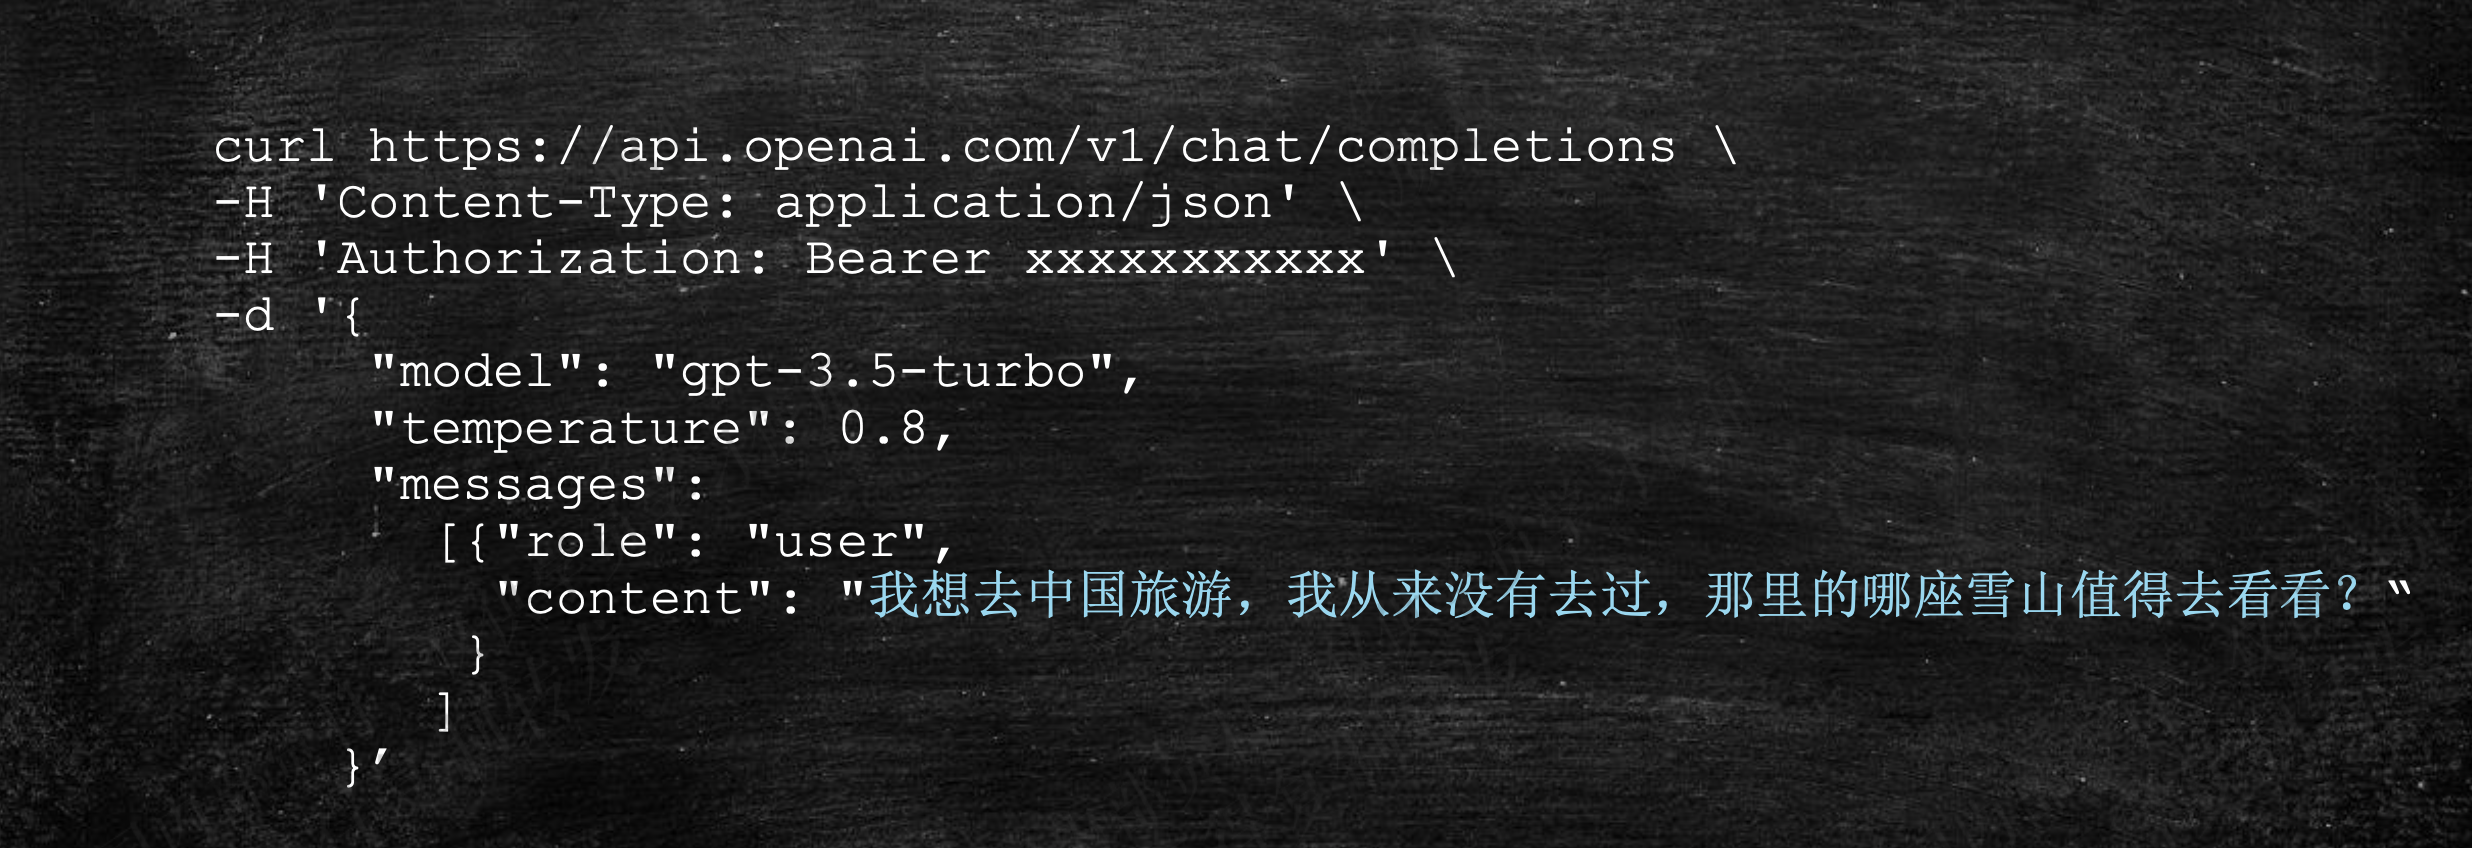
\includegraphics[width=0.6\textwidth]{figs/code.png}
\caption{“ChatGPT冰山下的”}
%\label{}
\end{figure}

\begin{figure}[htbp]
\centering
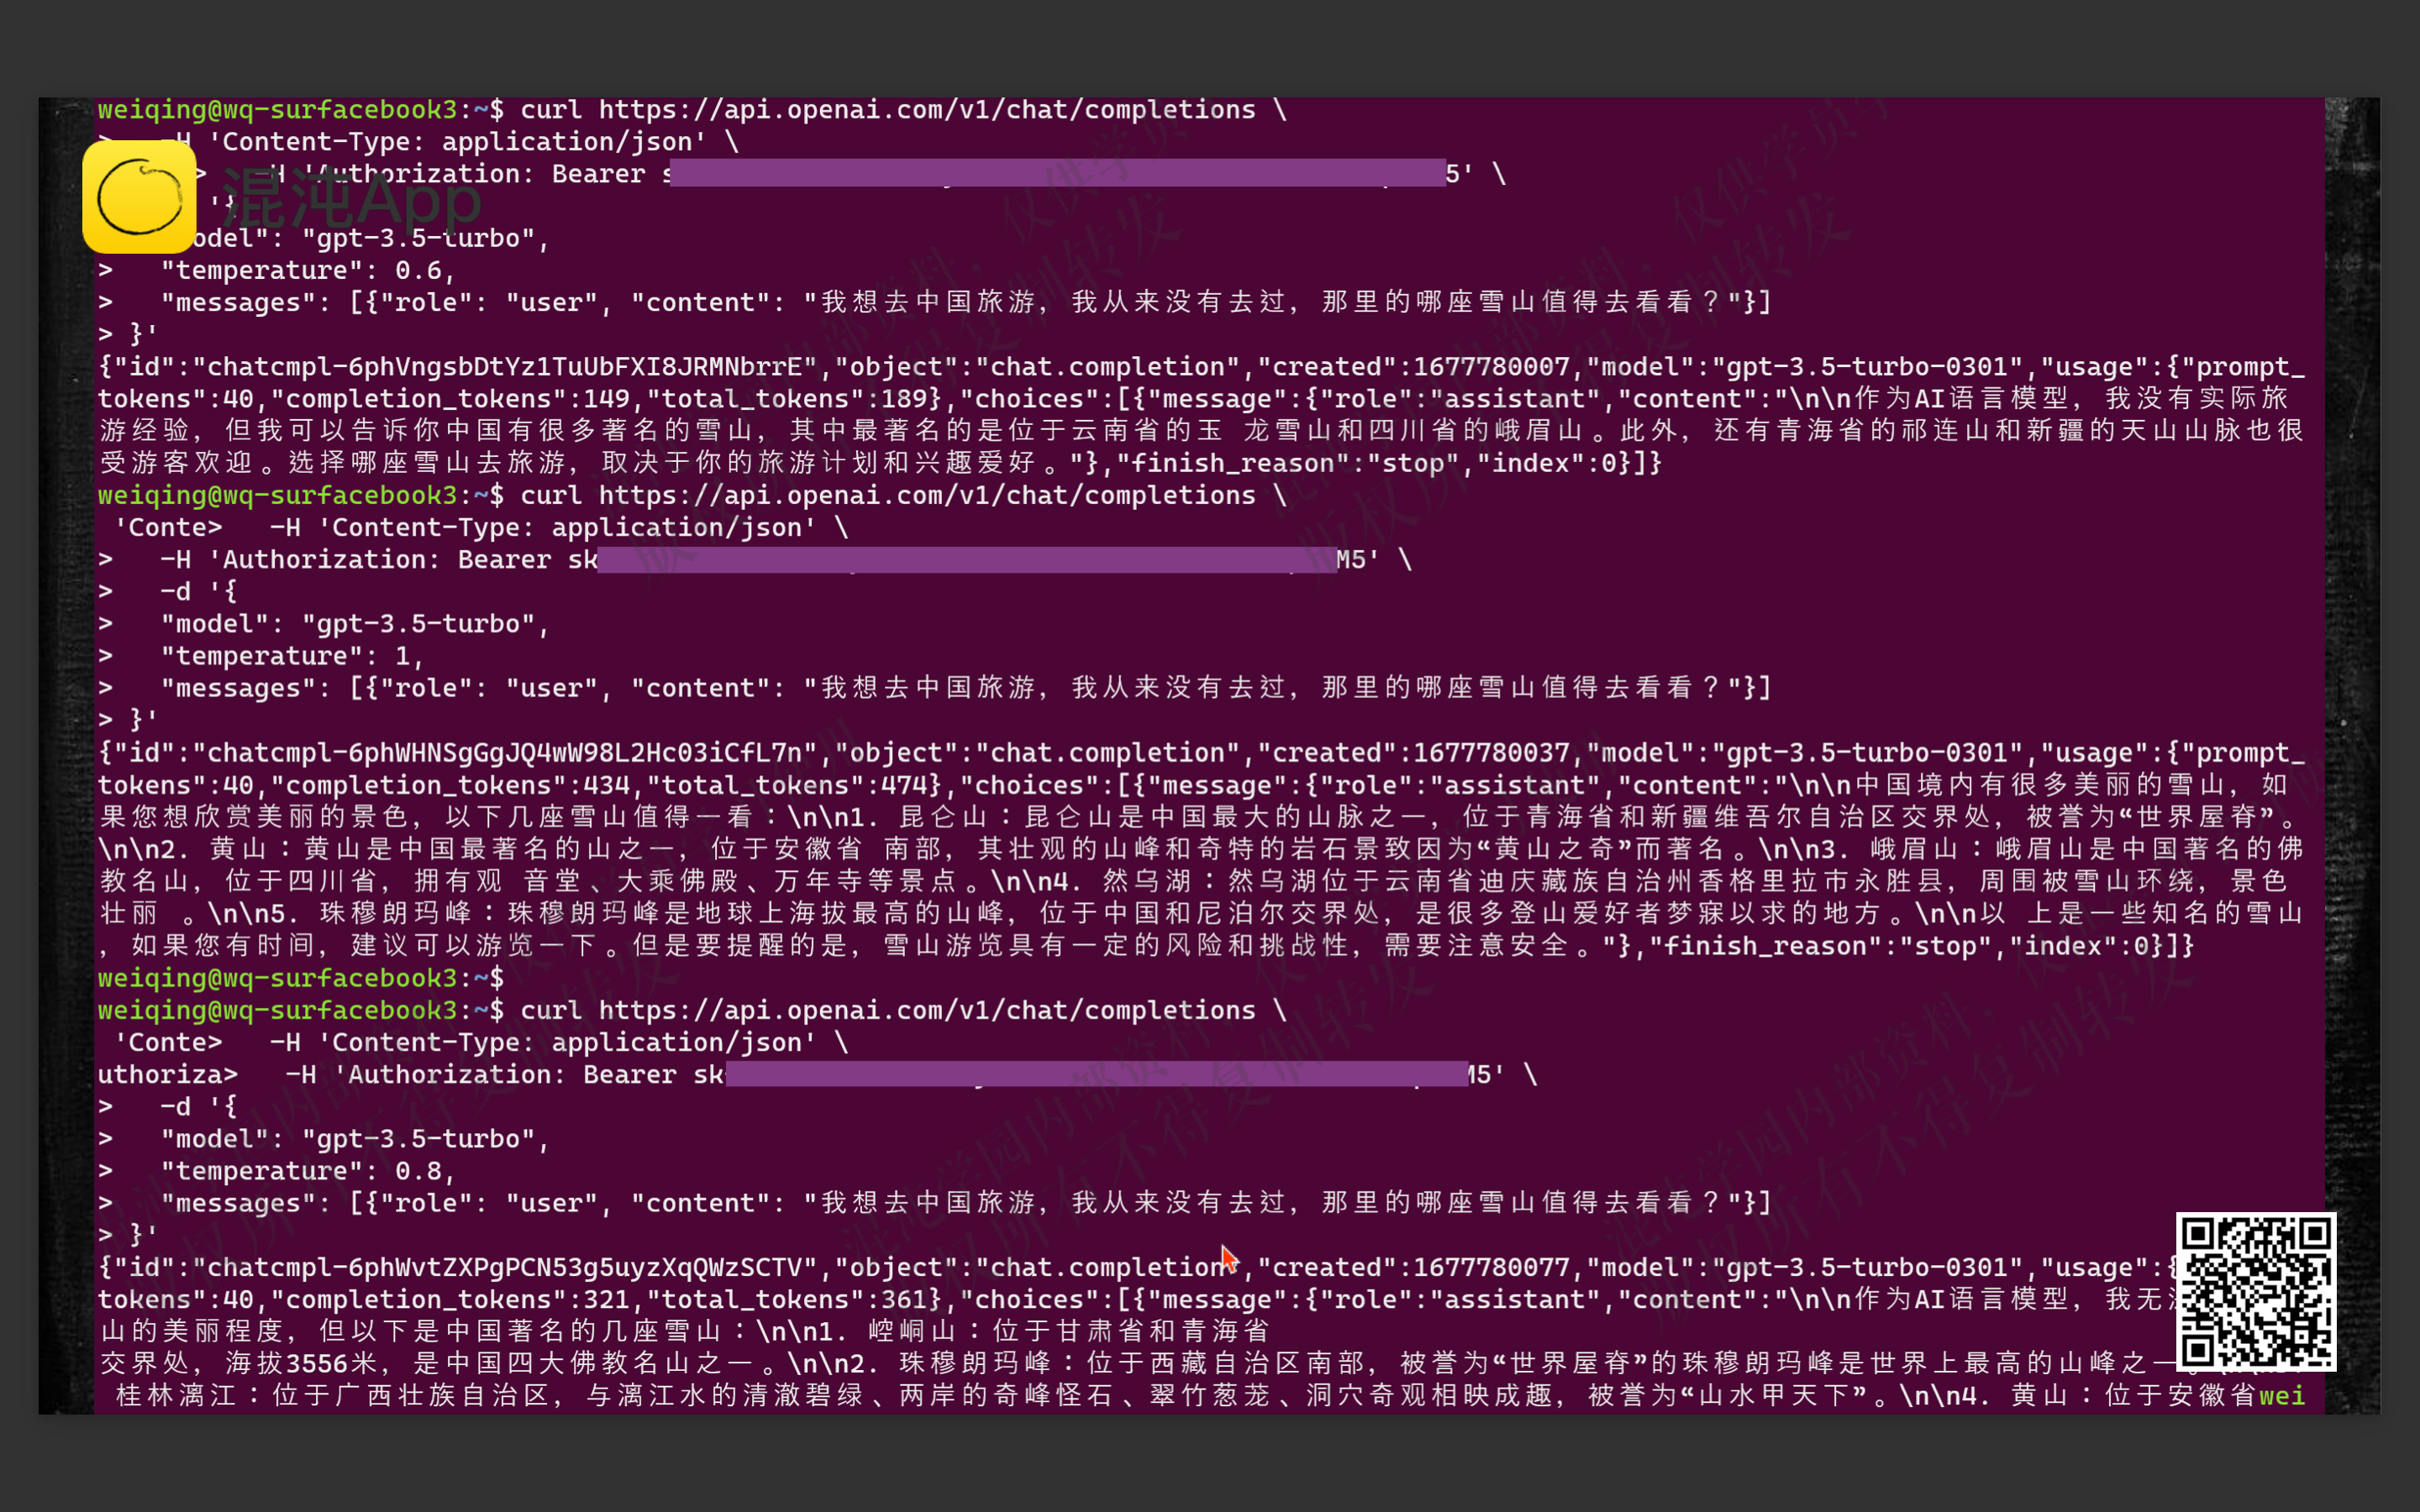
\includegraphics[width=0.6\textwidth]{figs/answer.png}
\caption{“ChatGPT冰山下的”}
%\label{}
\end{figure}


\begin{figure}[htbp]
\centering
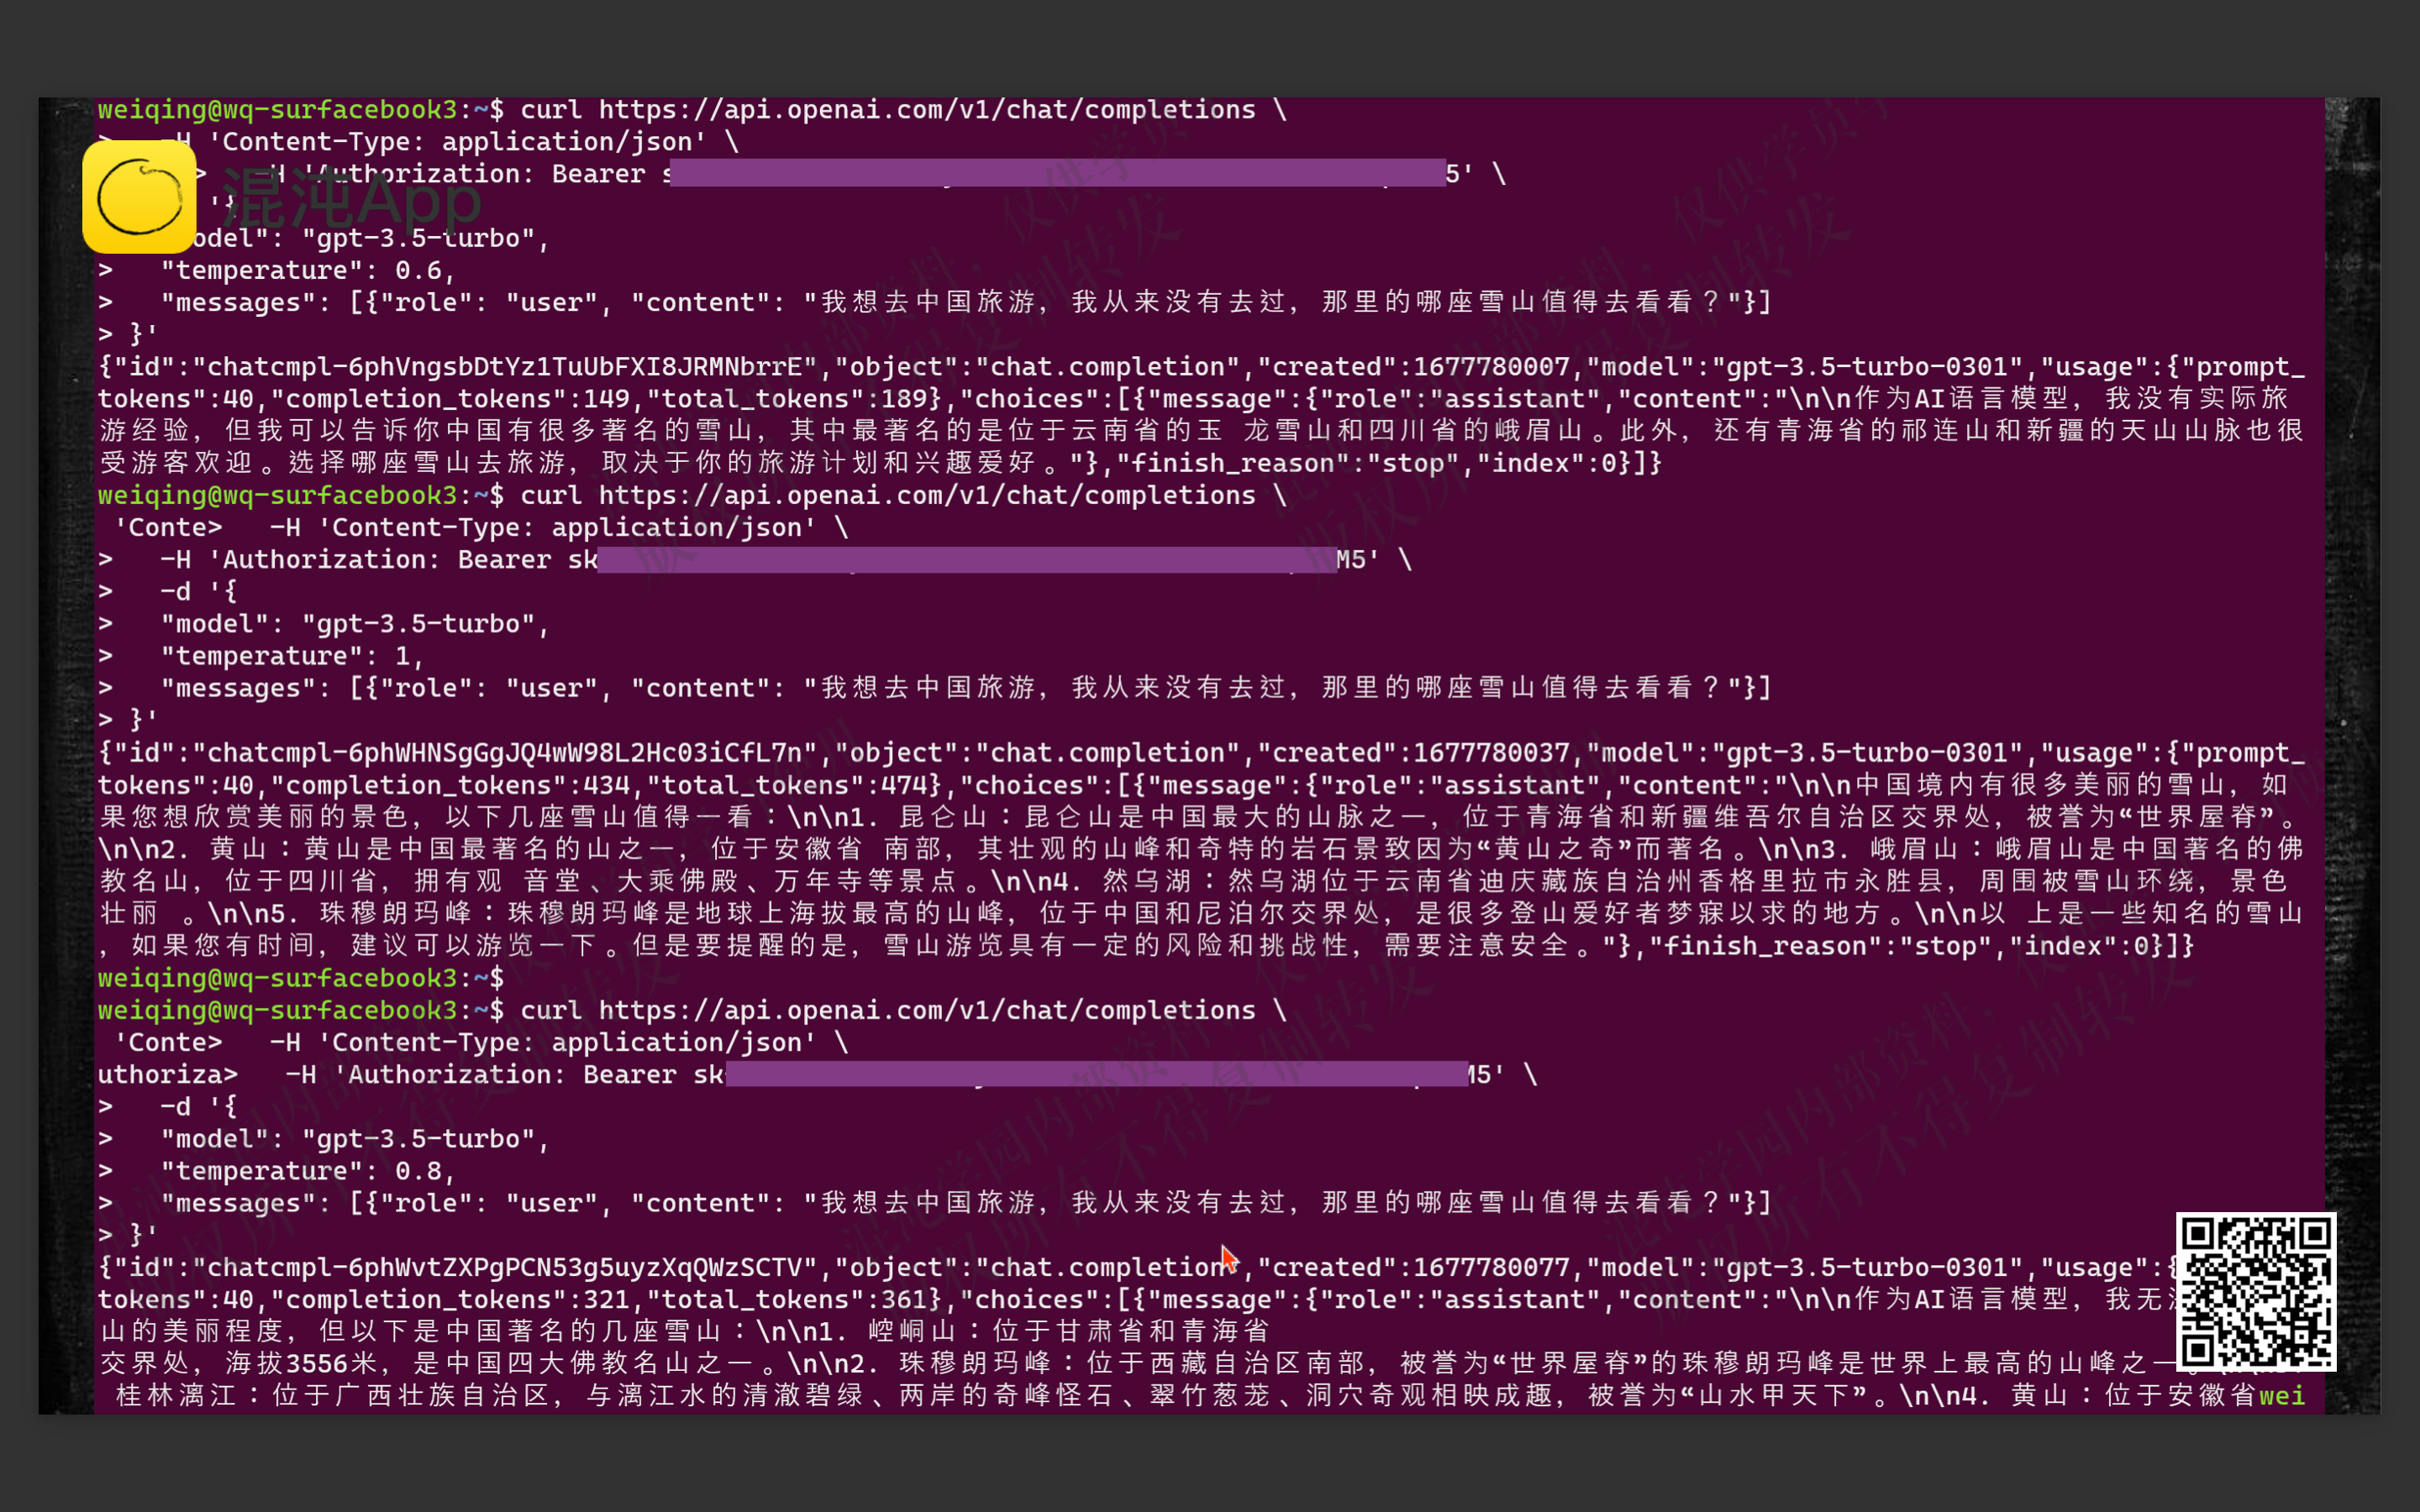
\includegraphics[width=0.6\textwidth]{figs/answer.png}
\caption{“我想去中国旅游，我从来没有去过，那里的哪座雪山值得去看看?”}
%\label{}
\end{figure}

\begin{figure}[htbp]
\centering
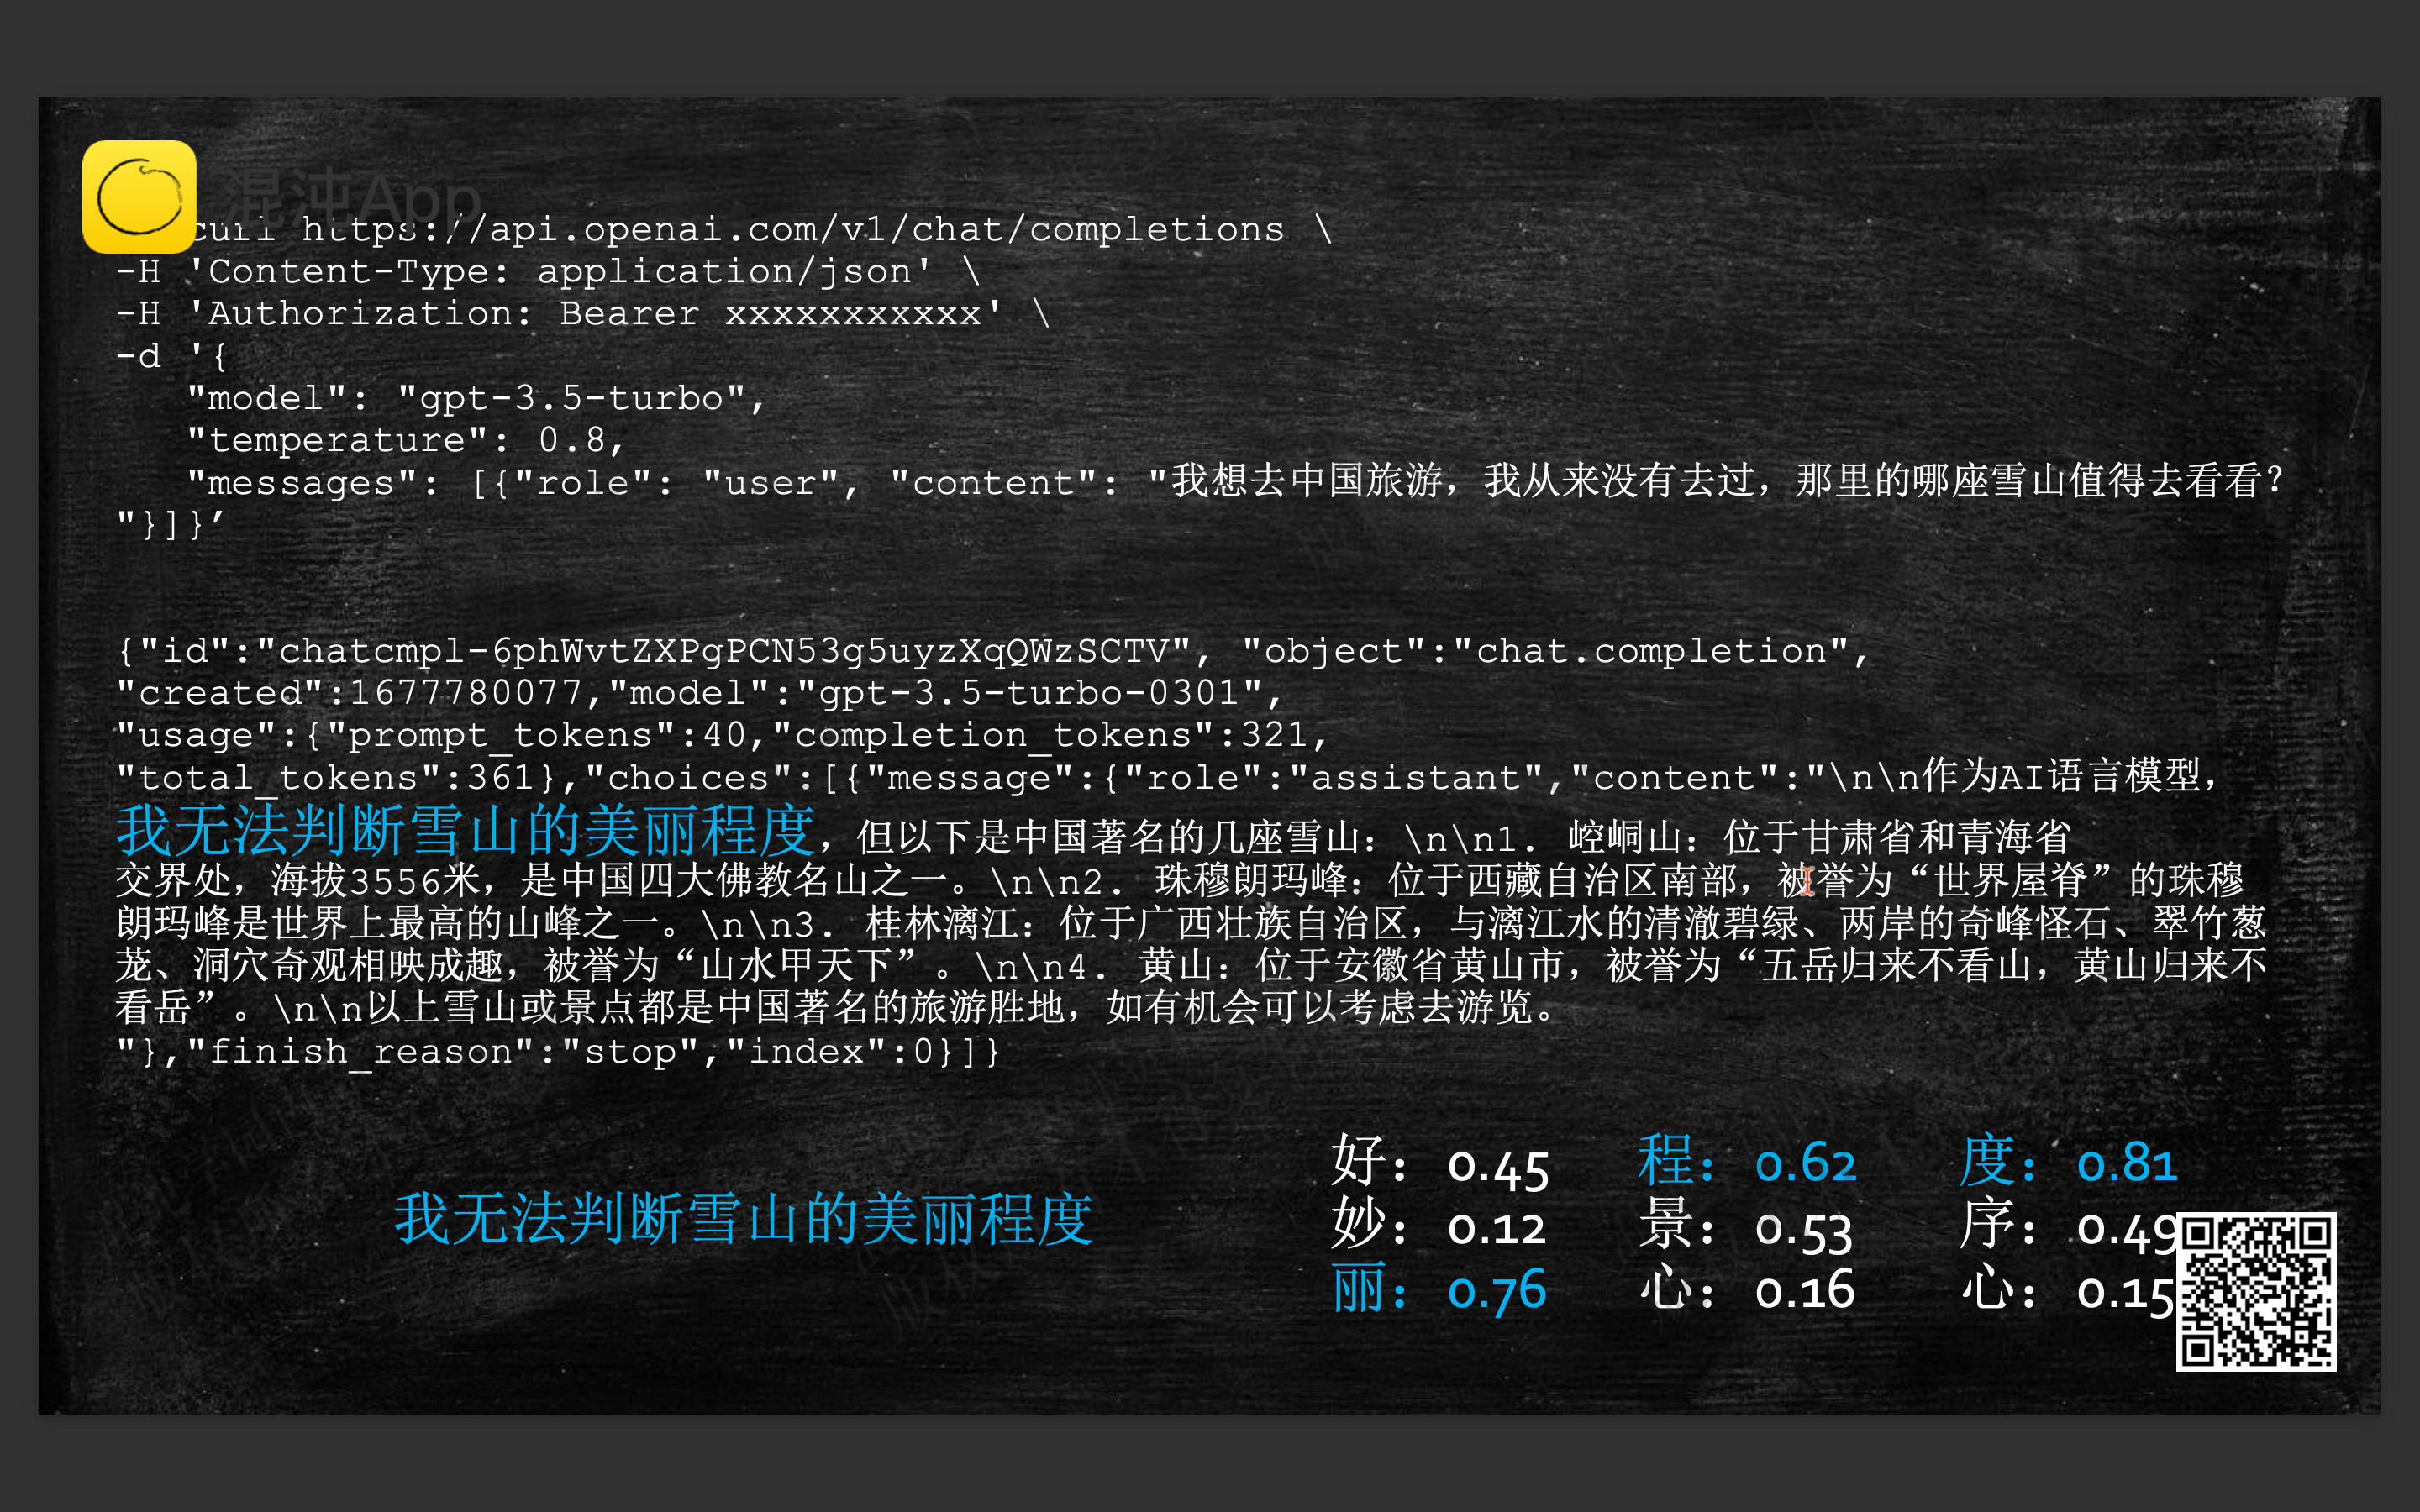
\includegraphics[width=0.6\textwidth]{figs/probability.png}
\caption{“我无法判断雪山的美丽程度”}
%\label{}
\end{figure}


\begin{figure}[htbp]
\centering
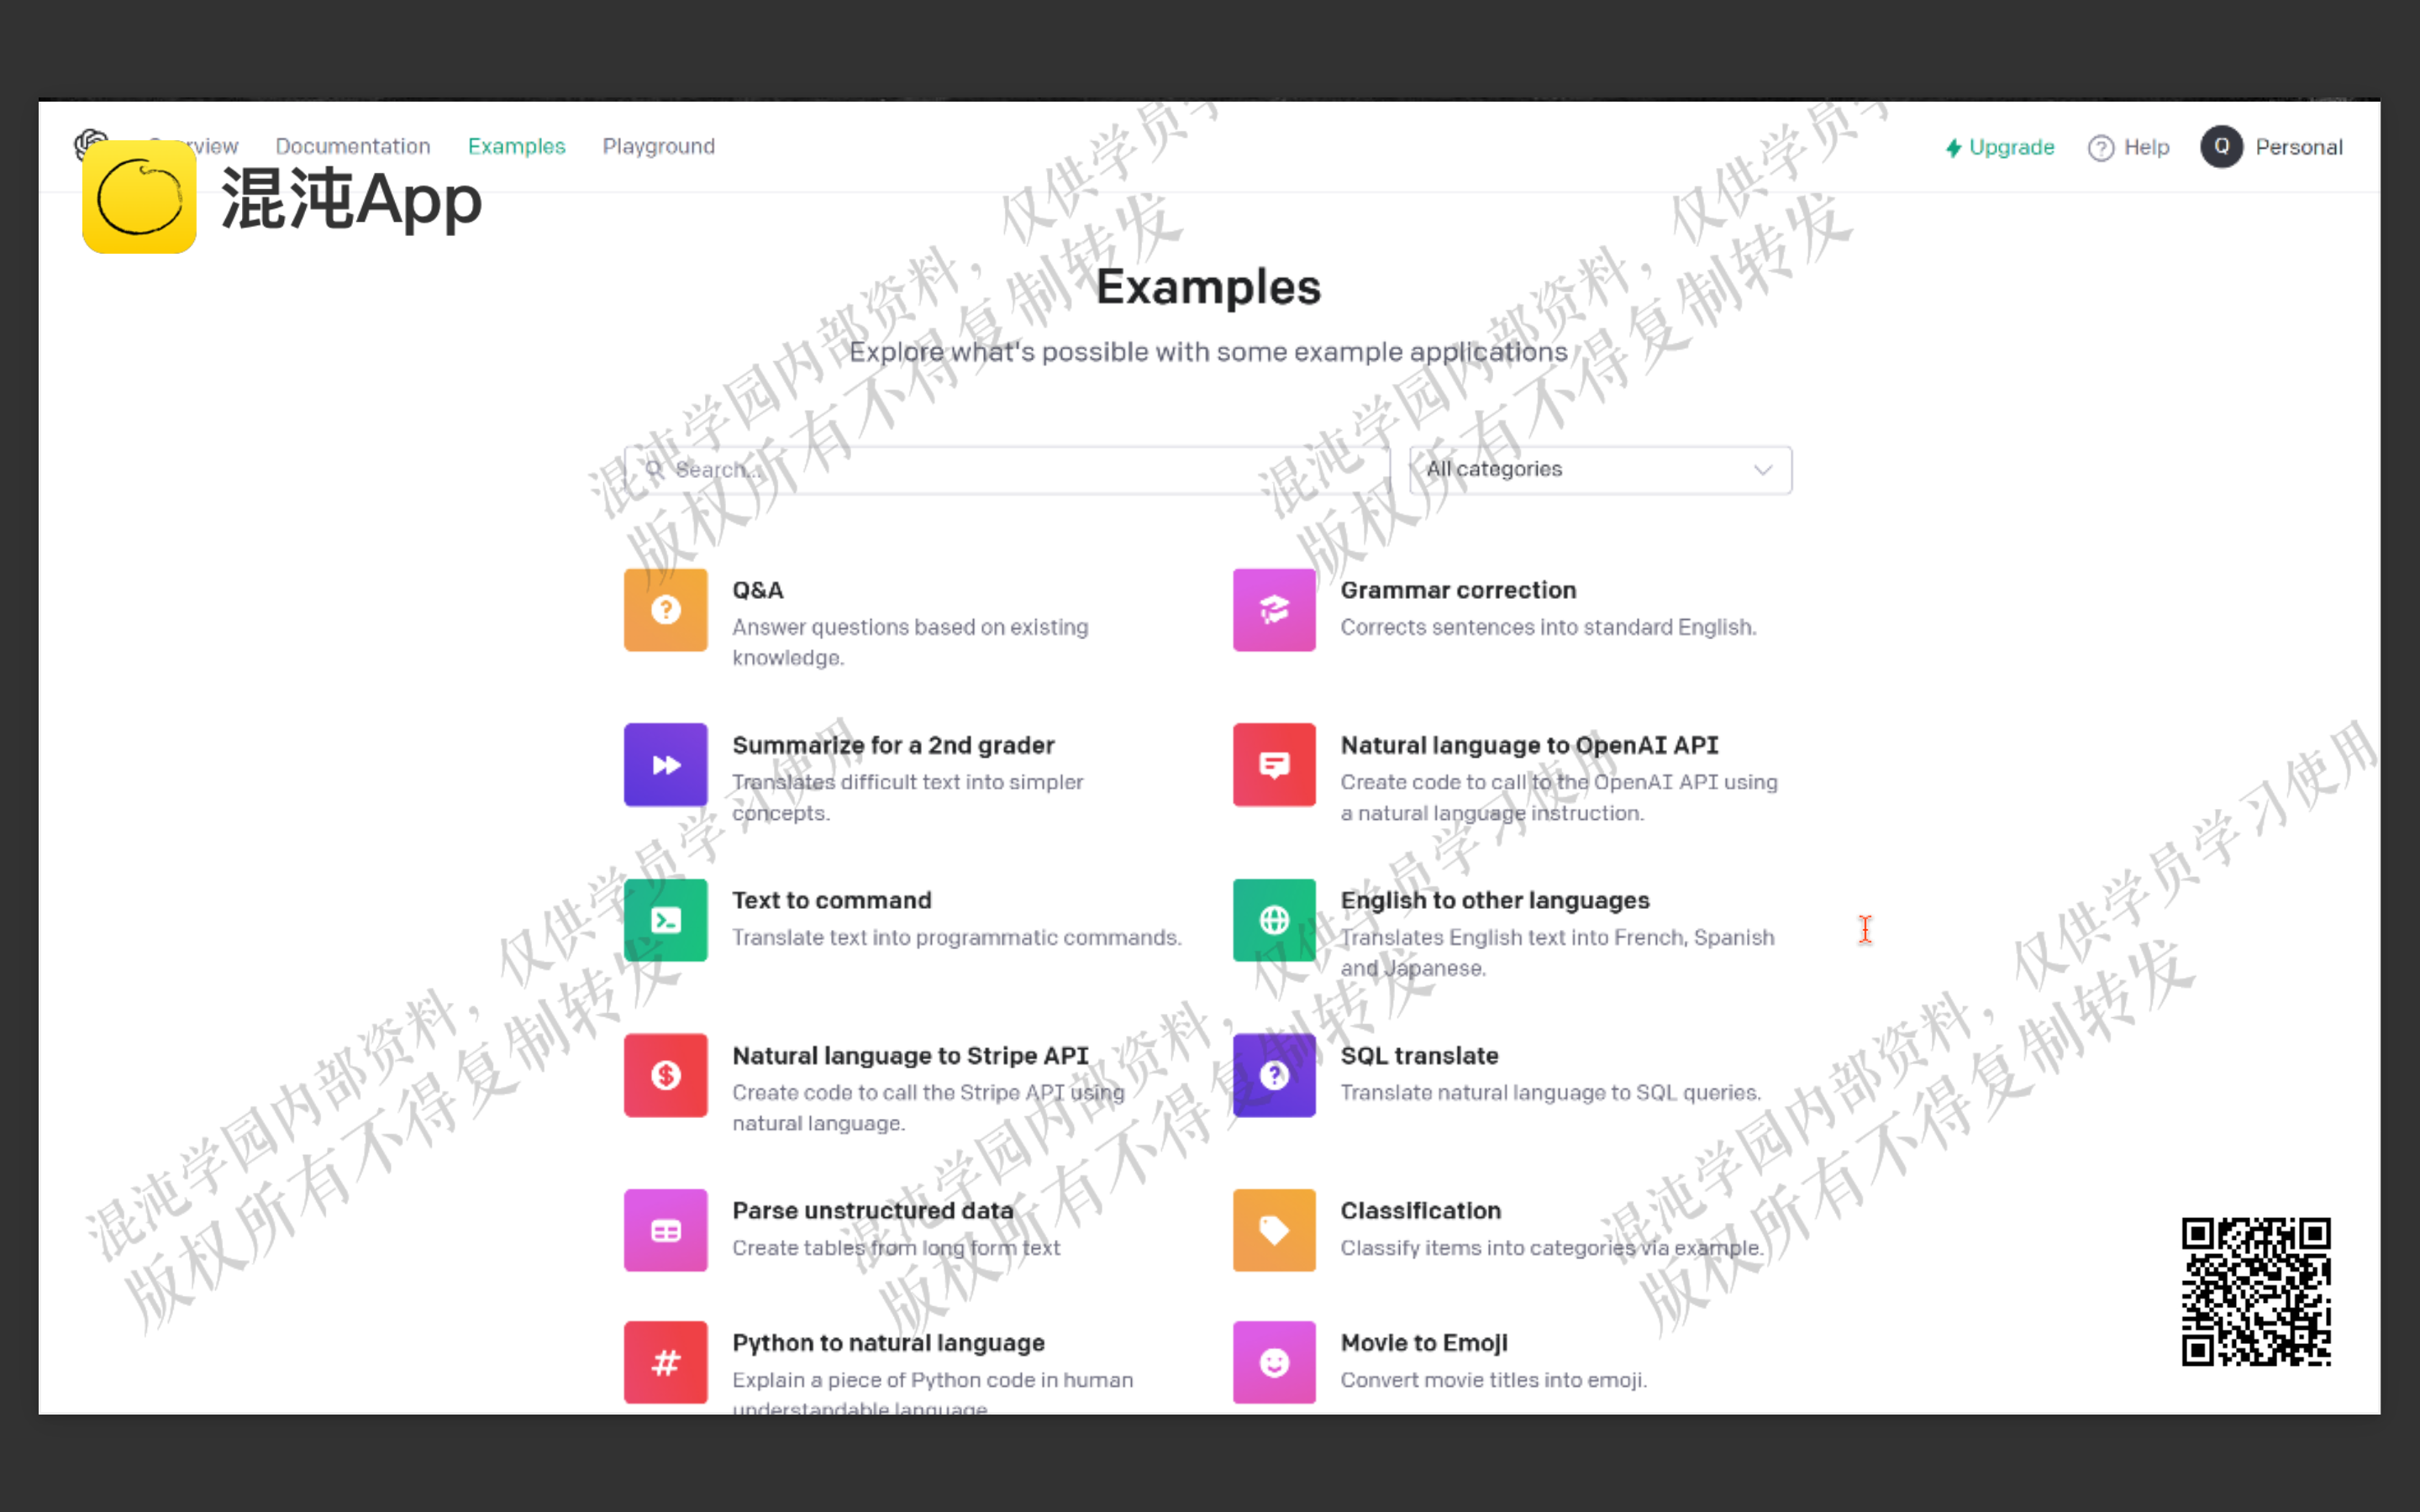
\includegraphics[width=0.6\textwidth]{figs/applications.png}
\caption{“ChatGPT冰山下的”}
%\label{}
\end{figure}

机器不理解概念， 
机器“理解”的是{\bf 概率分布 }
不是{\bf 概念推理}，{\bf 是概率推理}


看上去像人一样， 
不是机器像人， 
是人时常忽略何以为人

越是纷纷扰扰， 
越要守住第一性原理， 
始终回归初心
 

\begin{figure}[htbp]
\centering
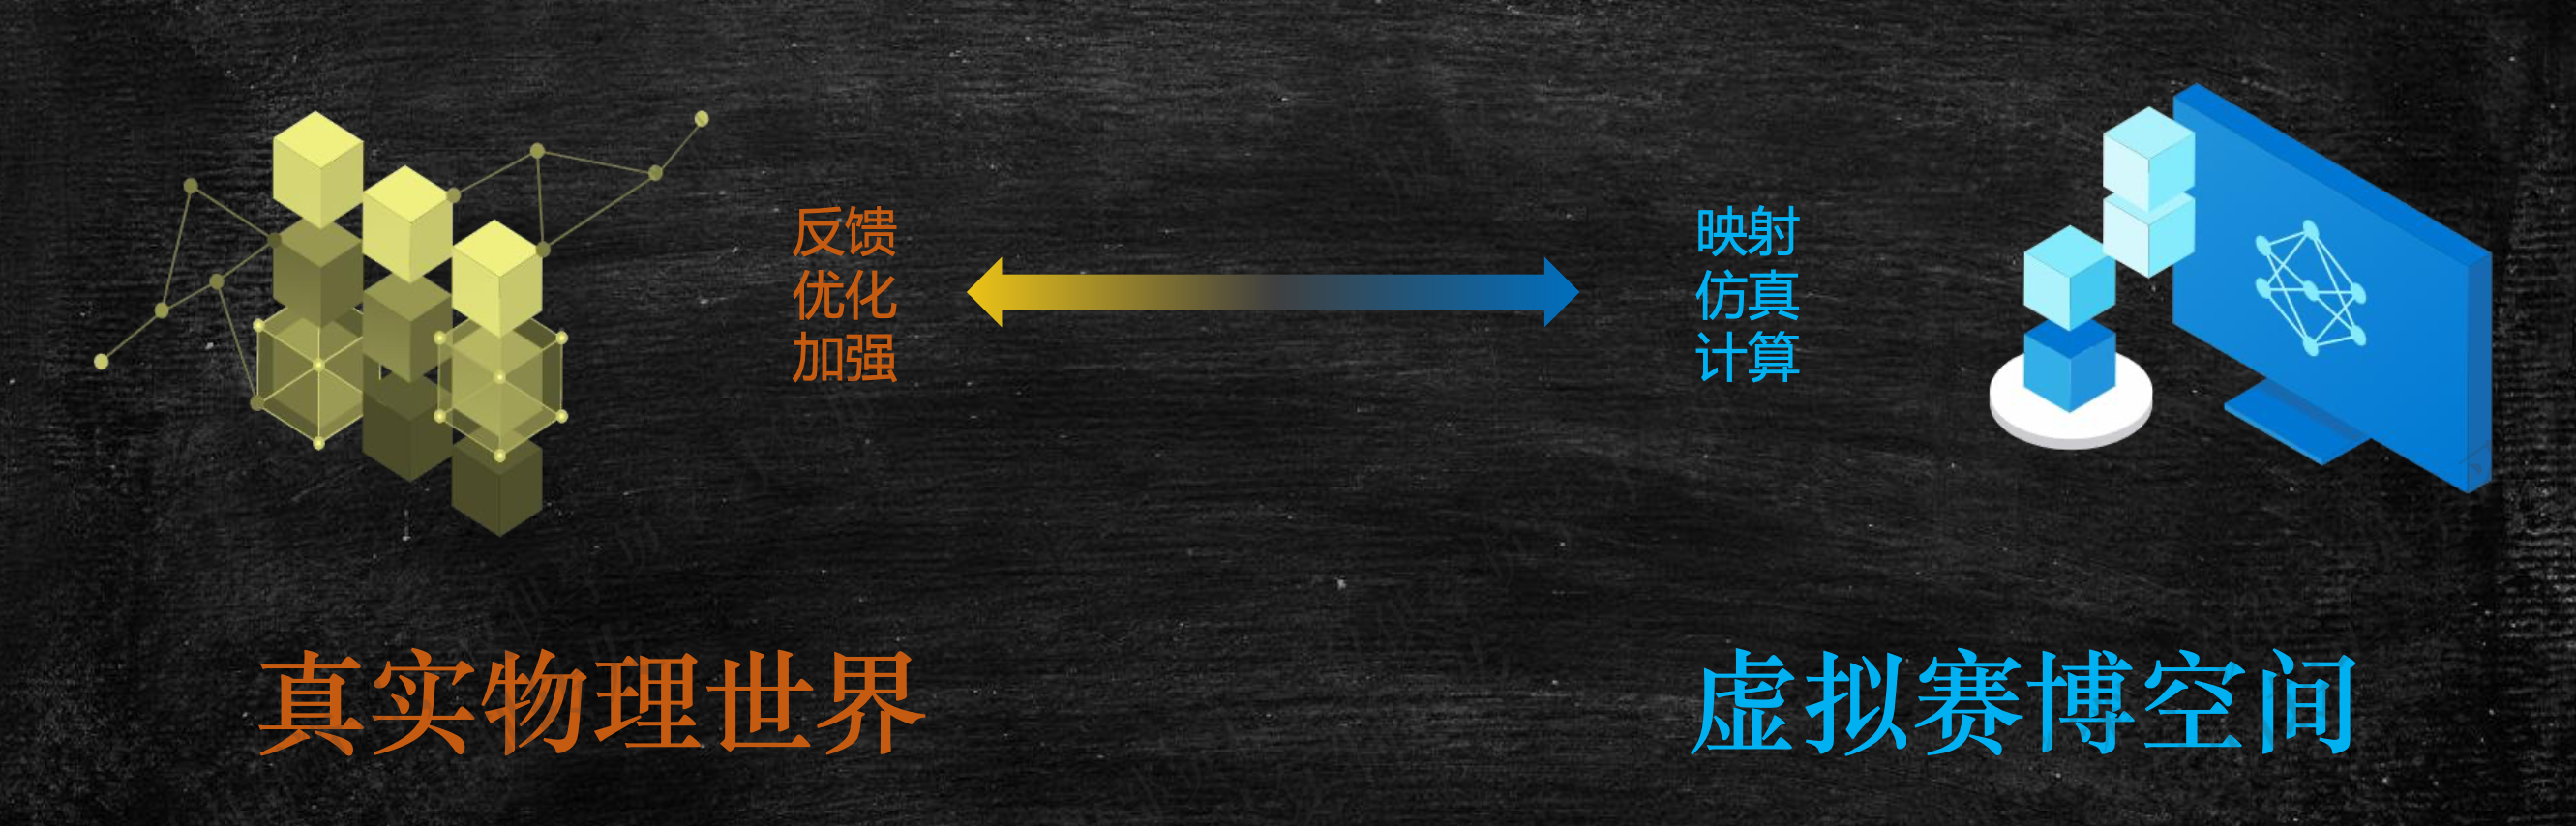
\includegraphics[width=0.6\textwidth]{figs/real_vs_cyber.png}
\caption{真实物理世界 v.s. 虚拟赛博空间}
%\label{}
\end{figure}

\begin{itemize}
\item 理解机器的运行机制，才能成为机器的主人
\begin{itemize}
\item  机器“蒸馏”人类知识
\item 人类学会教机器做事
 \end{itemize}
%\item  全流程再造，全流程赋能 
%\item 全员升级，全员赋能
\end{itemize}

信息商 （ Information Quotient）
\begin{enumerate}
\item 1. Critical but not cynical 时时审辩又不必事事怀疑
\item 2. System thinking 系统思维
\item 3. Signified v.s. Signifier 区分“所指”与“能指”
\item 4. Understand v.s Know 区分“理解”与“知道”
\item 5. Inverse, always inverse 反向思维
\item 6. Verification $\&$ Validation“验证”与“确认”
\item 7. Be aware of cognitive bias 随时审视“思维偏差”
\item 8. Develop a Bayes brain 培养贝叶斯大脑
\item 9. Master of machine 成为机器的主人
\item 10. Keep learning 终身学习
\end{enumerate}

提炼知识的算法没有文明，但被提炼的知识有文明

举例说明。 

未来地球的球籍，其中一个要素是
  各个文明对人类知识的贡献
  
- 初看是技术，细看全是人的问题 - 而人的最大问题是思想的问题

- 在确定性消失的时代，思想上的最大问题是以为按照确定性的方法可以解决不确定性的问题


常有人问:哪些人类工作会受到机器的影响? 或许应问:哪些人类工作不会受到机器的影响?

在一个机器既可以随时帮你，又可以随时“骗你”的时代 {\bf “何以为人”}成为一个根本问题

“动荡时代的最大风险不是动荡本身， 而是企图以昨天的逻辑来应对动荡
The greatest danger in times of turbulence is not the turbulence; it is to act with yesterday’s logic.”
— 彼得·德鲁克 Peter F. Drucker

 \section{对未来人类的影响}
1. 教育 – 允许“抄袭”的开卷考试 – 学会抄也是不容易的

2. 人类文明的再一次“重生Renaissance”-因信息流通而造成的再 一次知识平权

3. “认识你自己”-从体力竞争，到记忆力竞争，再到思维力竞争 - 人类可能高估了知识的复杂性，又低估了思想的深刻性


{\bf 人-机关系 Homo Sapiens – Machina Sapiens}

1. 机器弥补人类的弱点 
2. 人类指挥机器





\nocite{*}
\printbibliography[heading=bibintoc, title=\ebibname]

\newpage